\begin{tikzpicture}[transform shape]
	% Define coordinates for the main elements
	\coordinate (leftImg) at (0,0);
	\coordinate (topImg) at (4.5,2.5);
	\coordinate (bottomImg) at (4.5,-2.5);
	\coordinate (rightEq) at (10,0.25);

	% Place the placeholder images (blue rectangles with numerical solution)
	\node[inner sep=0] (leftRectangle) at (leftImg)
	{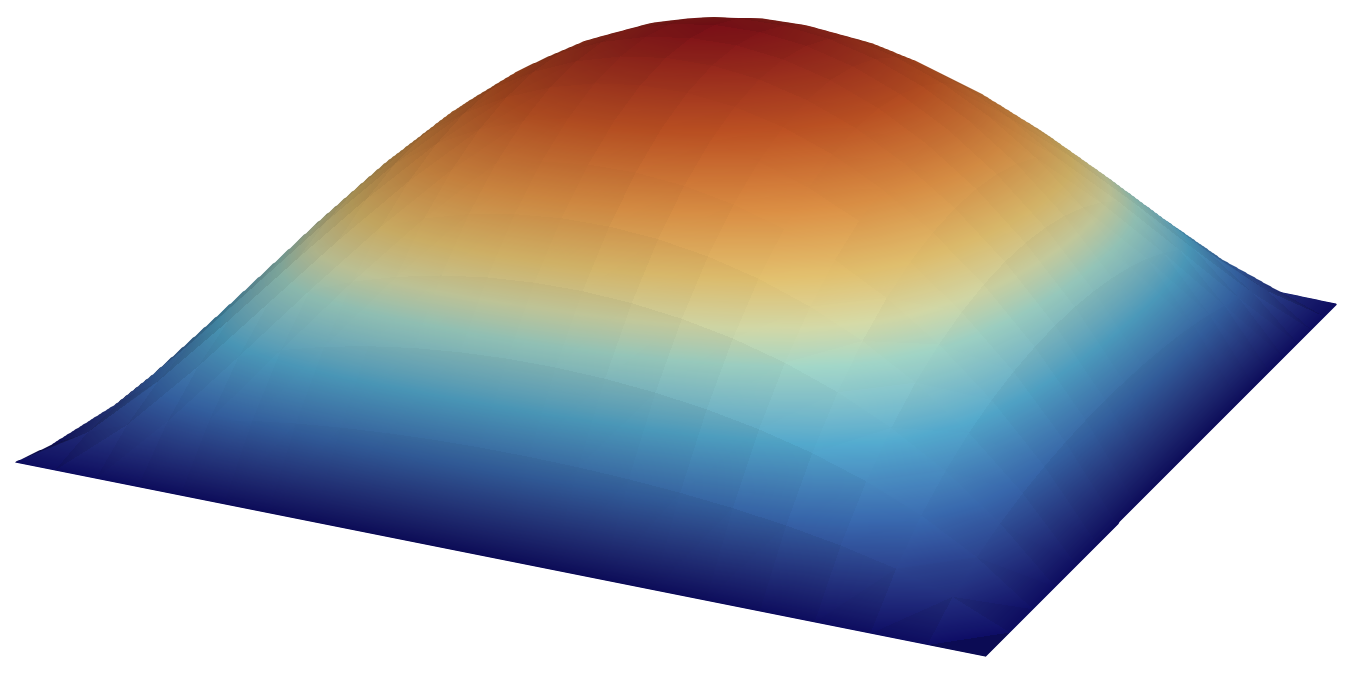
\includegraphics[width=5cm]{images/global-solution.png}};
	\node[inner sep=0] (topRectangle) at (topImg)
	{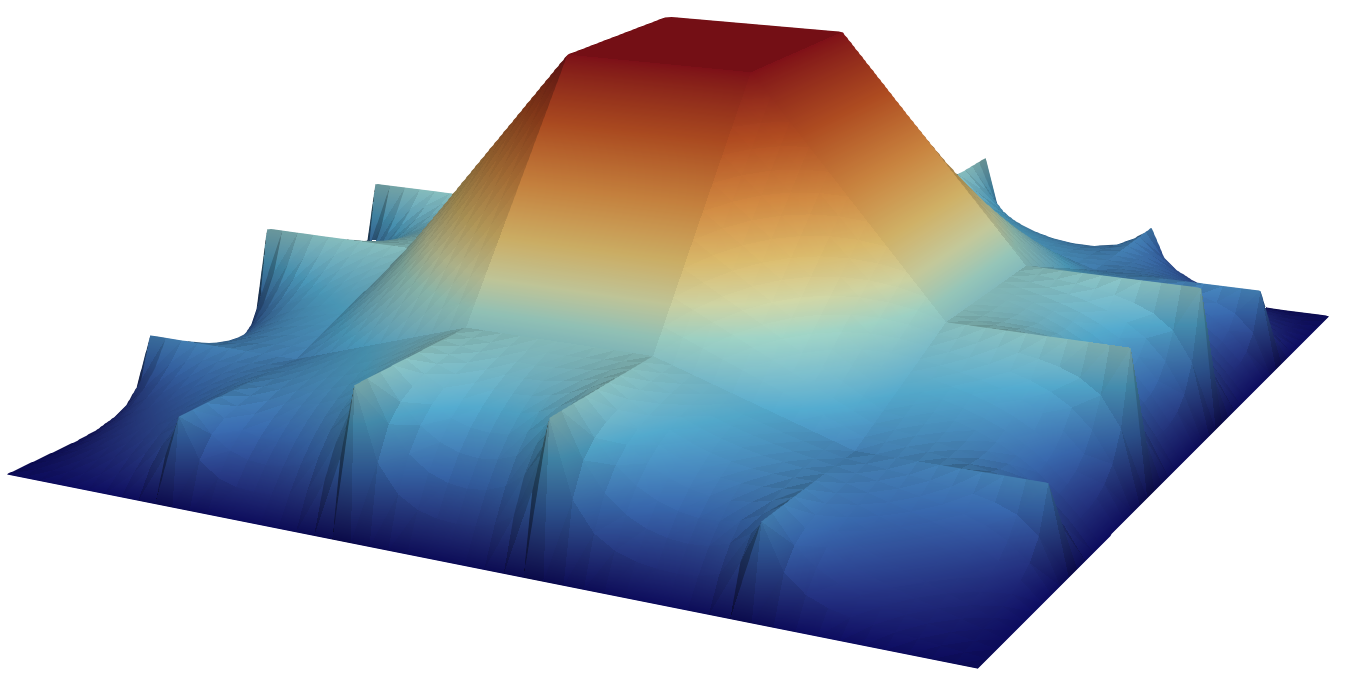
\includegraphics[width=5cm]{images/coarse-solution.png}};
	\node[inner sep=0] (bottomRectangle) at (bottomImg)
	{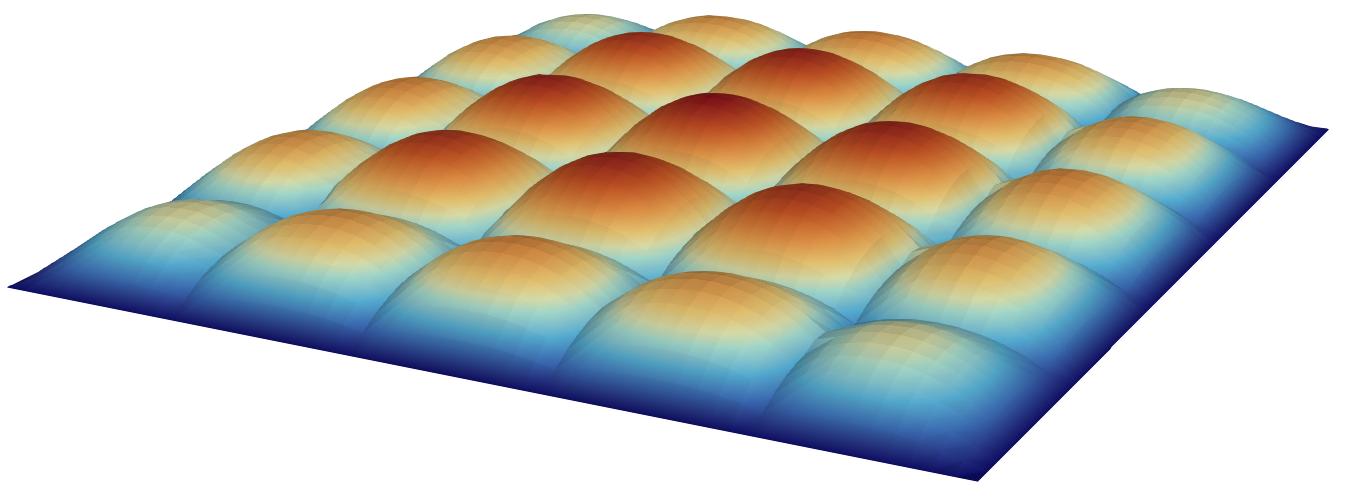
\includegraphics[width=5cm]{images/local-solutions.png}};

	\node[yshift=0mm, xshift=-10mm, text width = 35mm, font=\small] at (leftRectangle.north) {Discretized nonlinear problem};
	\node[yshift=-0mm, xshift=-10mm, font=\small] at (leftRectangle.south) {$F(u) = 0$};

	\node[yshift=-2mm, font=\small] at (bottomRectangle.south) {$R_i F\left(u - P_i T_i(u)\right) = 0$};

	\node [yshift=-2mm, font=\small] at (topRectangle.south){$\varPhi^T F\left(u - \varPhi T_0(u)\right) = 0$};

	% \node[align=left, text width = 4.5cm, font=\small] at (9.5,-1.9){Solve with Newton's method for nonlinear corrections $T_i(u) \text{ for } i = 1,2,\dots,N$};

	\node[draw, rectangle, text width = 4.9cm, minimum height=1cm, font=\small]
    (boxedEq) at (rightEq) {\begin{equation*}\begin{split}&\mathcal{F}_H(u) = \\&\sum_{i=1}^{N} P_i T_i(u-\varPhi T_0(u)) + \varPhi T_0(u)\\&\quad\quad = 0\end{split}\end{equation*}};

	% Arrows
	\draw[-{Stealth[length=3mm, width=2mm]}] ($(leftRectangle.north) + (1.3, -0.2)$) -- ($(topRectangle.south west) + (0.1, 0.6)$);
	\draw[-{Stealth[length=3mm, width=2mm]}] ($(leftRectangle.south east) + (-1.1, 0.0)$) -- ($(bottomRectangle.north west) + (1.0, -0.4)$);
	\draw[-{Stealth[length=3mm, width=2mm]}] ($(topRectangle.south east)+ (-0.4, 0.9)$) -- ($(boxedEq.north west)+ (-0.1, 0.1)$);
	\draw[-{Stealth[length=3mm, width=2mm]}] ($(bottomRectangle.north east)+ (-0.8, -0.1)$) -- ($(boxedEq.south west)+ (-0.1, -0.1)$);
\end{tikzpicture}
